\chapter{\LaTeX}\label{app:latex}
\begin{quote}
    {\it If you want your mathematical writing to look like real math then the modern
    mathematician uses \LaTeX\ for all of their writing.}
\end{quote}
\LaTeX\ is a powerful mathematical typesetting language.  We encourage students to use a
tool such as Overleaf (\href{https://www.overleaf.com/}{https://www.overleaf.com/}) to do
their \LaTeX\ editing.  Overleaf is an online platform much like Google Docs where you can
write and share dynamically in real time.  In this appendix we give the basics of mathematical writing with \LaTeX.  


\section{Equation Environments and Cross Referencing}

When working with equations is it often times convenient and necessary to cross-reference
the equations that you're talking about.  A simple example is:
\begin{example}\label{ex:C2:pythag}
    Recall the Pythagorean Theorem: If $a$ and $b$ are the legs of a right triangle and
    $c$ is the hypotenuse, then
    \begin{flalign}
        a^2 + b^2 = c^2.
        \label{eqn:pythag}
    \end{flalign}

    Let $a=3$ and $b=4$ in equation \eqref{eqn:pythag}. If that is the case then \dots

    The \LaTeX\ code for this is \index{flalign} \index{label} \index{eqref}
\begin{verbatim}
Recall the Pythagorean Theorem: If $a$ and $b$ are the legs of a 
right triangle and $c$ is the hypotenuse, then
\begin{flalign}
    a^2 + b^2 = c^2 
    \label{eqn:pythag}
\end{flalign}

Let $a=3$ and $b=4$ in equation \eqref{eqn:pythag}. 
If that is the case then \dots
\end{verbatim}
\end{example}

Note in Example \ref{ex:C2:pythag} that the equations and the equation reference are part
of the sentence.  In fact, these are always part of the grammatical structure of your
writing.  



Other numbered environments include \texttt{align, flalign, eqnarray, equation} and
several others.  The modern convention for \LaTeX\ is to use \texttt{align}  \index{align} or
\texttt{flalign} for all equations.  If you want to use one of these environments without
numbers then use the *.  In otherwords \texttt{align*} \index{align*} will align in the same way without
numbering the equations.  If you only want a number on one line then you can
use \verb|\notag| \index{equations without numbers} at the beginning of that line.

To align equations use the ``align" enviroment, which requires the amsmath package. Align
supersedes eqnarray. The ampersands control the vertical alignment:
\begin{verbatim}
\begin{align}
\frac{\partial{x}}{\partial{s}}&=zx  & \text{with} && x(0)=1\\
\frac{\partial{y}}{\partial{s}}&=x^2y & \text{with} && y(0)=t\\
\frac{\partial{z}}{\partial{s}}&=xyz & \text{with} && z(0)=t^2
\end{align}
\end{verbatim}

\begin{align}
\frac{\partial{x}}{\partial{s}}&=zx  & \text{with} && x(0)=1\\
\frac{\partial{y}}{\partial{s}}&=x^2y & \text{with} && y(0)=t\\
\frac{\partial{z}}{\partial{s}}&=xyz & \text{with} && z(0)=t^2
\end{align}



A few more math-related typesetting examples are included below:
\begin{itemize}


    \item Inline math with and without numbering \index{equations without numbers}
        \index{square brackets} \index{flalign} \index{label} \index{subequations}

        \begin{verbatim}
        \[ \sum_{j=1}^\infty \frac{1}{j^2} = \frac{\pi^2}{6} \]
        \end{verbatim}
        \[ \sum_{j=1}^\infty \frac{1}{j^2} = \frac{\pi^2}{6} \]

        \begin{verbatim} 
        \begin{flalign}
            \sum_{j=1}^\infty \frac{1}{j^2} = \frac{\pi^2}{6}
            \label{eqn:sample_equation}
        \end{flalign}
        \end{verbatim}
        \begin{flalign}
            \sum_{j=1}^\infty \frac{1}{j^2} = \frac{\pi^2}{6}
            \label{eqn:sample_equation}
        \end{flalign}

        \begin{verbatim}
        \begin{subequations}
            \begin{eqnarray}
                \sin \left( \frac{\pi}{6} \right) &=& \frac{\sqrt{3}}{2}
                \label{eqn:sine} \\
                \cos \left( \frac{\pi}{6} \right) &=& \frac{1}{2}
                \label{eqn:cosine}
            \end{eqnarray}
            \label{eqn:trig}
        \end{subequations}
        \end{verbatim}
        \begin{subequations}
            \begin{eqnarray}
                \sin \left( \frac{\pi}{6} \right) &=& \frac{\sqrt{3}}{2}
                \label{eqn:sine} \\
                \cos \left( \frac{\pi}{6} \right) &=& \frac{1}{2}
                \label{eqn:cosine}
            \end{eqnarray}
            \label{eqn:trig}
        \end{subequations}
        This second example allows you to cross reference equations \index{cross
        reference} \index{eqref} \index{ref} like
        (\ref{eqn:sample_equation}) using
        \verb|(\ref{eqn:sample_equation})| or, more simply, \eqref{eqn:sample_equation}
        using \verb|\eqref{eqn:sample_equation}|. The third set of equations
        allows for multiple types of references.  Like: \\
        The sine equation, \eqref{eqn:sine} \verb|(\eqref{eqn:sine})|, and the cosine equation,
        \eqref{eqn:cosine} \verb|(\eqref{eqn:cosine})|, are grouped together via equation
        \eqref{eqn:trig} \verb|(\eqref{eqn:trig})|.





    \item Matrices \index{matrix} \index{matrix!pmatrix} \index{matrix!vmatrix}
        \index{matrix!bmatrix}

        \begin{minipage}{3.5in}
\begin{verbatim}
    \[ \begin{bmatrix} 1 & 2 \\ 3 & 4 \end{bmatrix} \]
\end{verbatim}
\begin{verbatim}
    \[ \begin{pmatrix} 1 & 2 \\ 3 & 4 \end{pmatrix} \]
\end{verbatim}
\begin{verbatim}
    \[ \begin{vmatrix} 1 & 2 \\ 3 & 4 \end{vmatrix} \]
\end{verbatim}
        \end{minipage}
        \begin{minipage}{3in}
            \[ \begin{bmatrix} 1 & 2 \\ 3 & 4 \end{bmatrix} \]
            \[ \begin{pmatrix} 1 & 2 \\ 3 & 4 \end{pmatrix} \]
            \[ \begin{vmatrix} 1 & 2 \\ 3 & 4 \end{vmatrix} \]
        \end{minipage}

    \item Including basic graphics \\ \index{graphics} \index{graphics!file type}
        \index{graphics!includegraphics}
        Be sure that the graphics file is in the same directory as your TeX
        file. Your picture should be a *.eps or *.pdf file. If not then some TeX
        compilers will complain (plus, *.jpg usually looks horrible).
\begin{verbatim}
    \begin{center}
        \includegraphics[width=0.9\columnwidth]{filename.eps}
    \end{center}
\end{verbatim}
OR
\begin{verbatim}
    \begin{center}
        \includegraphics[height=3in]{filename.eps}
    \end{center}
\end{verbatim}
        There are many options for \verb|\includegraphics|, but these two
        work for many pictures.  Sometimes, though, it is desired to trim an image that
        you've saved from elsewhere.  The basic syntax for \texttt{trim} and \texttt{clip}
        \index{trim and clip} is
\begin{verbatim}
    \begin{center}
        \includegraphics[trim = 1cm 2cm 1cm 2cm, clip=true, 
            width=0.9\columnwidth]{filename.eps}
    \end{center}
\end{verbatim}
        The four measurements after the trim command are the amount to trim from the left,
        bottom, right, and top (in that order).




    \item Leaving white space:\index{white space}
        \begin{itemize}
            \item horizontal Spacing: \verb|\hspace{0.5in}|
            \item vertical Spacing: \verb|\vspace{2in}|
        \end{itemize}

\end{itemize}



\section{Tables, Tabular, Figures, Shortcuts, and Other Environments}

\subsection{Tables and Tabular Environments}
Tables can be rather annoying in \LaTeX, but it is important to get the basics down before
moving on.  \index{table} \index{table!tabular}

\begin{example}\label{ex:C3:tabular} In this example we want the table to be place {\it here} [h*], the
        first column left justified, the middle column centered, and the
        last column right justified with vertical bars between each column.
        \index{tabular}
        \begin{verbatim}
        \begin{center}
            \begin{tabular}[h*]{|l|c|r|}
                \hline
                Title 1 & Title 2 & Title 3 \\ \hline \hline
                Hello & Ni Hao & Bonjour \\ \hline
                good bye & zia jian & adieux \\ \hline
            \end{tabular}
        \end{center}
        \end{verbatim}
        \begin{center}
            \begin{tabular}[h*]{|l|c|r|}
                \hline
                Title 1 & Title 2 & Title 3 \\ \hline \hline
                Hello & Ni Hao & Bonjour \\ \hline
                good bye & zia jian & adieux \\ \hline
            \end{tabular}
        \end{center}
    \end{example}
In Example \ref{ex:C3:tabular} we used the tabular environment.  This builds the table.
If you want to build a table where there is a caption and the environment {\it floats} to
various parts of the page then you need to use the \texttt{table} command.  

\begin{example}\label{ex:C3:table} In this example we build the same table as in Example
    \ref{ex:C3:tabular} but this time we allow it to float and we want a caption.  The
    code is: \index{table} \index{table!caption} \index{table!label}
\begin{verbatim}
\begin{table}
    \centering
        \begin{tabular}[h*]{|l|c|r|}
            \hline
            Title 1 & Title 2 & Title 3 \\ \hline \hline
            Hello & Ni Hao & Bonjour \\ \hline
            good bye & zia jian & adieux \\ \hline
        \end{tabular}
    \caption{This is the amazing table of doom}
    \label{tab:MyLabel}
\end{table}
\end{verbatim}
\end{example}
    \begin{table}
        \begin{center}
            \begin{tabular}[h*]{|l|c|r|}
                \hline
                Title 1 & Title 2 & Title 3 \\ \hline \hline
                Hello & Ni Hao & Bonjour \\ \hline
                good bye & zia jian & adieux \\ \hline
            \end{tabular}
        \end{center}
        \caption{This is the amazing table of doom}
        \label{tab:MyLabel}
    \end{table}



\subsection{Excel To \LaTeX}
One tool that is often overlooked is the \texttt{ExcelToLaTeX} macro for Excel.  I'm
leaving this one up to you.  Google \texttt{ExcelToLaTeX} \index{Excel to LaTeX}, download
it, add it to the macros for your version of Excel, and have fun with it.  This tool will
allow you to convert Excel-based tables to \LaTeX\ tables.





\subsection{Figures}
\index{figure}
The \texttt{figure} environment in \LaTeX\ is almost identical to that for \texttt{table}.
For example:
\begin{example}\label{ex:C3:fig}
This figure simply shows a MatLab plot of the sine and cosine functions together in all of
their shared glory.  The file type was \texttt{eps}, which is notoriously hard to handle
on Windows machines and on Overleaf.  Be sure to use the \texttt{epstopdf} package if
you're using \texttt{eps}file types.  \index{figure!caption} \index{figure!label}
\index{figure!placement}
\begin{verbatim}
\begin{figure}[ht!]
    \centering
    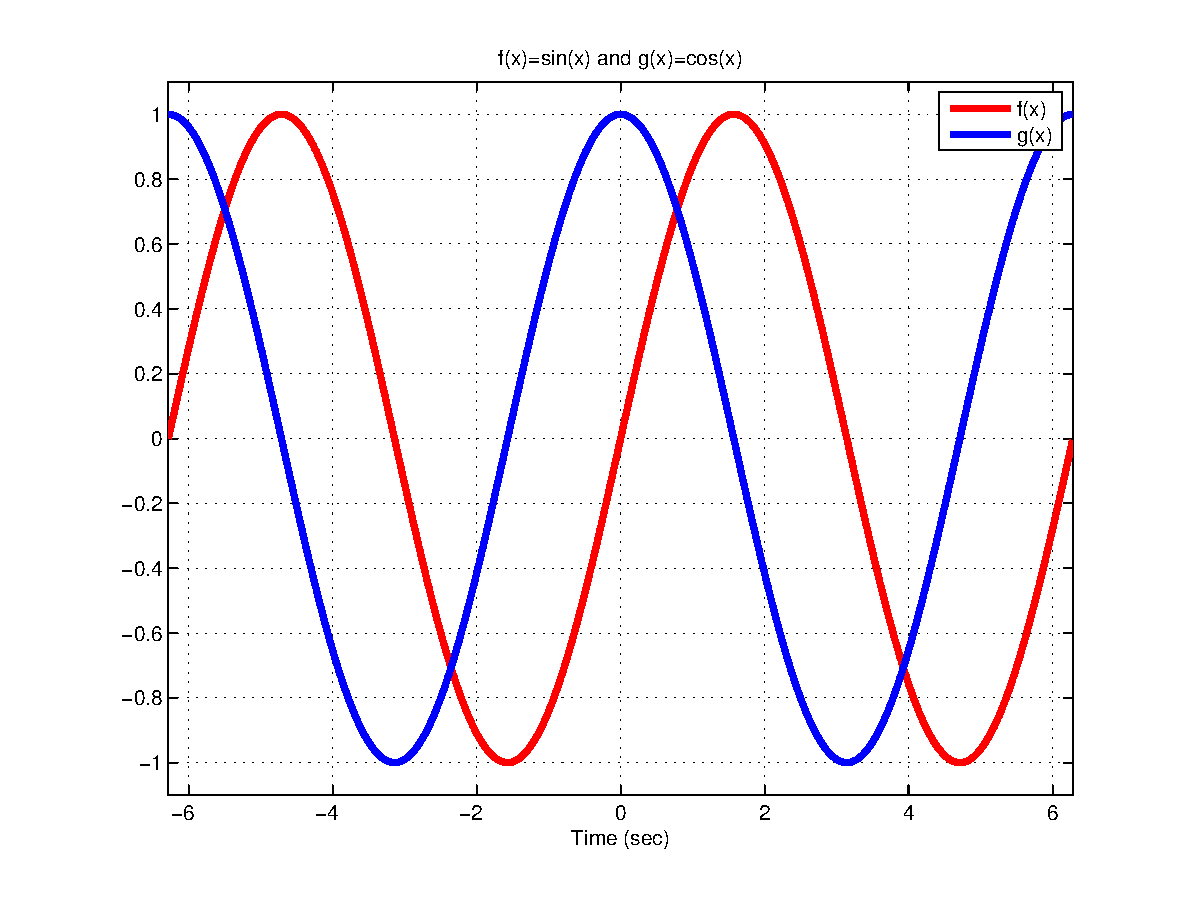
\includegraphics[width=0.7\columnwidth]{SampleFigure.eps}
    \caption{Figure for Example \ref{ex:C3:fig}
    \label{fig:C3:fig}
\end{figure}
\end{verbatim}
\end{example}
    \begin{figure}[ht!]
        \begin{center}
            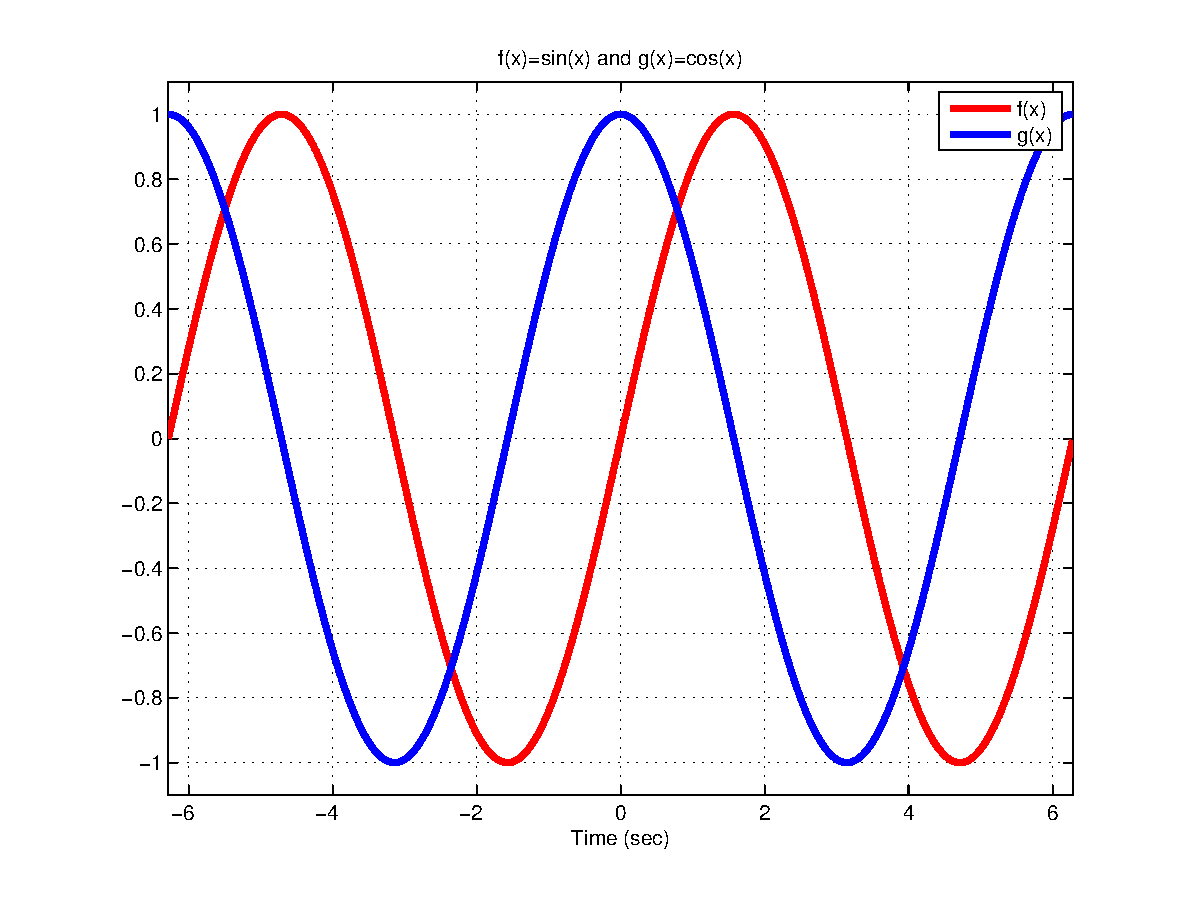
\includegraphics[width=0.7\columnwidth]{SampleFigure.eps}
        \end{center}
        \caption{Figure for Example \ref{ex:C3:fig}}
        \label{fig:C3:fig}
    \end{figure}



\subsection{New Commands: Shortcuts are AWESOME!}
You can save yourself a vast amount of typing by defining new commands which meet your
specific need. It is easy. The \texttt{newcommand} \index{newcommand} command goes in the preamble (before
the \verb|\begin{document}|). The examples that follow are a few handy ones that I've used
in the past.  The world is your oyster here, so make any shortcut for a \LaTeX\ command
that is cumbersome to type.
\begin{itemize}
    \item Derivatives
\begin{verbatim}
\newcommand{\dd}[2] {\frac{d #1}{d #2}}
\newcommand{\ddd}[2] {\frac{d^2 #1}{d #2^2}}

\dd{y}{x}
\ddd{y}{x}
\end{verbatim}

The results are:\\
\[\dd{y}{x}\]
\[\ddd{y}{x}\]

\item Partial derivatives
\begin{verbatim}
\newcommand{\pd}[2] {\frac{\partial{#1}}{\partial{#2}}}
\newcommand{\pdd}[2] {\frac{\partial^2{#1}}{\partial{#2}^2}}
\newcommand{\pddm}[3] {\frac{\partial^2{#1}}{\partial{#2}\partial{#3}}}

\pd{y}{x}
\pdd{y}{x}
\pddm{y}{x}{z}
\end{verbatim}

The results are:\\
\[\pd{y}{x}\]
\[\pdd{y}{x}\]
\[\pddm{y}{x}{z}\]

\item Some of the common number sets
\begin{verbatim}
\newcommand{\cc}{\mathbb{C}}
\newcommand{\rr}{\mathbb{R}}
\newcommand{\nn}{\mathbb{N}}
\newcommand{\qq}{\mathbb{Q}}
\newcommand{\zz}{\mathbb{Z}}

\cc \hspace{1cm} \nn \hspace{1cm} \qq \hspace{1cm} \rr \hspace{1cm} \zz
\end{verbatim}
The result is:
\[\cc \hspace{1cm} \nn \hspace{1cm} \qq \hspace{1cm} \rr \hspace{1cm} \zz\]

\item Grouping symbols (parentheses, brackets, etc) \index{grouping!parenthesis}
    \index{grouping!brackets}
\begin{verbatim}
\newcommand{\lp}{\left(}
\newcommand{\rp}{\right)}
\newcommand{\lb}{\left[}
\newcommand{\rb}{\right]}

\lp\pdd{F}{x}\rp
compared to
(\pdd{F}{x})
\end{verbatim}

The result is:
\[\lp\pdd{F}{x}\rp\]
compared to
\[(\pdd{F}{x})\]

\item Common conjunctions
\begin{verbatim}
\newcommand{\andd}[1]{\quad\text{and}\quad}
\newcommand{\orr}[1]{\quad\text{or}\quad}
\newcommand{\forr}[1]{\quad\text{for}\quad}
\newcommand{\st}[1]{\quad\text{such that}\quad}
\newcommand{\conj}[1]{\quad\text{#1}\quad}

% Implies
\newcommand{\ra}{\quad\Rightarrow\quad}

A\ra B\st C\ne D
\end{verbatim}

The result is:
\[A\ra B\st C\ne D\]
\end{itemize}



\section{Graphics in \LaTeX}
In this chapter we will focus on several tools that extend your knowledge of figures
beyond just \texttt{includegraphics} and move you toward the domain of professional
publications.  The tools that we'll cover are:\index{graphics!tikz}
\index{graphics!pgfplots} \index{graphics!GeoGebra}  \index{graphics!MatLab}
\begin{enumerate}
    \item The \texttt{tikz} package,
    \item The \texttt{pgfplots} package,
    \item Using \texttt{GeoGebra} to generate \texttt{tikz} code, and 
    \item Using \texttt{MatLab} to generate \texttt{tikz} code.
\end{enumerate}

These tools take a lot of work, but the end result is well worth it.  
\begin{center}
    {\bf There is nothing worse or more distracting than a poorly done figure.}
\end{center}

There is more to these packages than we could possibly cover in a few days.  It is
imperative that you use the internet to its fullest extent with these packages.  You can
get yourself into a pickle with some of the internet-based examples, but starting with someone
else's code for these packages is \"uber helpful sometimes!

What I'll present here are simply a few examples to get you going.

\subsection{The Tikz and PGFPlots Packages}
The Tikz package is made for doing line drawings.  The simplest mode of operation with
Tikz is to do point-by-point drawings on a Cartesian grid.
\begin{example}
    Say we want to draw a coordinate plane with a few geometric shapes.  Inside the
    \texttt{figure} environment we include a \texttt{tikzpicture} environment around the
    code for the picture.  Be sure to end every Tikz line with a semicolon;  Figure
    \ref{fig:C5:tikz1} shows the results. \index{graphics!draw}
    \index{graphics!tikzpicture}
\begin{verbatim}
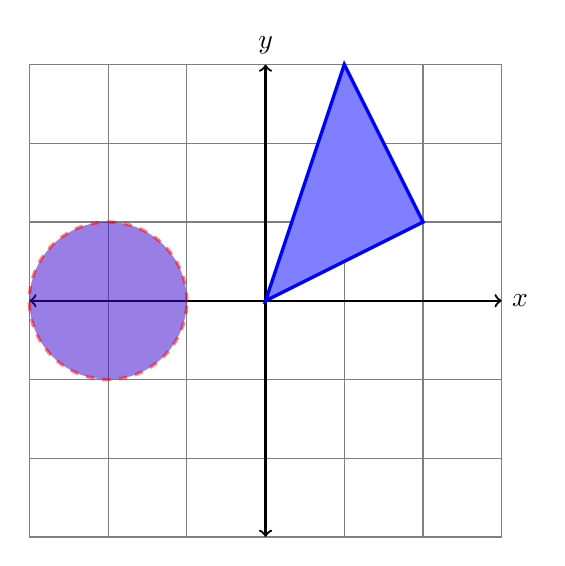
\begin{tikzpicture}
    \draw[color=gray] (-3,-3) grid (3,3);
    \draw[thick, <->] (-3,0) -- (3,0) node[anchor=west]{$x$};
    \draw[thick, <->] (0,-3) -- (0,3) node[anchor=south]{$y$};
    \draw[very thick, blue, fill=blue!50] (0,0) -- 
        (2,1) -- (1,3) -- cycle;
    \draw[very thick, dashed, color=red, 
        fill=red!20!blue, opacity=0.5] (-2,0) circle(1cm);
\end{tikzpicture}
\end{verbatim}
\end{example}
    \begin{figure}[ht!]
        \begin{center}
            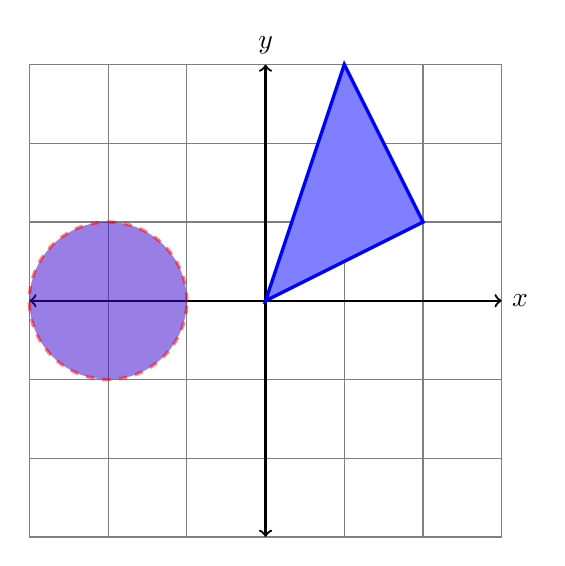
\begin{tikzpicture}
                \draw[color=gray] (-3,-3) grid (3,3);
                \draw[thick, <->] (-3,0) -- (3,0) node[anchor=west]{$x$};
                \draw[thick, <->] (0,-3) -- (0,3) node[anchor=south]{$y$};
                \draw[very thick, blue, fill=blue!50] (0,0) -- (2,1) -- (1,3) -- cycle;
                \draw[very thick, dashed, color=red, fill=red!20!blue, opacity=0.5] (-2,0) circle(1cm);
            \end{tikzpicture}
        \end{center}
        \caption{A simple Tikz picture}
        \label{fig:C5:tikz1}
    \end{figure}

For more examples about the Tikz package, see
\href{http://www.texample.net/tikz/examples/}{http://www.texample.net/tikz/examples/}
\dots texample \index{texample} is your new best friend.




You don't have to plot in MatLab, Excel, or any other tool when writing a technical
document!  Say this to yourself 100 times and be sure that you're sitting down.

\begin{example}
    This first example shows a simple way to plot functions. \index{graphics!axis}
    \index{graphics!addplot} \index{graphics!addlegendentry}
\begin{verbatim}
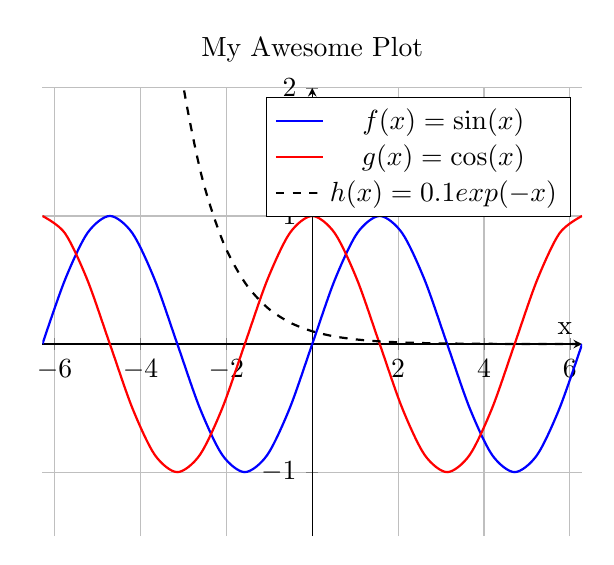
\begin{tikzpicture}
    \begin{axis}[axis lines=center, xlabel={x}, 
            title={My Awesome Plot},
            domain=-2*pi:2*pi, ymin=-1.5, ymax=2, grid]
        \addplot[blue, thick, smooth] {sin(deg(x))};
        \addlegendentry{$f(x)=\sin(x)$};
        \addplot[red, thick, smooth] {cos(deg(x))};
        \addlegendentry{$g(x)=\cos(x)$};
        \addplot[black, dashed, thick, smooth] {0.1*exp(-x)};
        \addlegendentry{$h(x)=0.1\text{exp}(-x)$};
    \end{axis}
\end{tikzpicture}
\end{verbatim}
\end{example}
    \begin{figure}[ht!]
        \begin{center}
            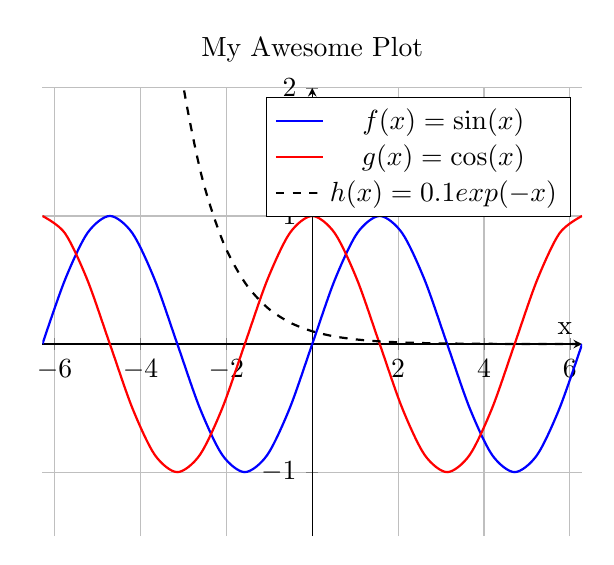
\begin{tikzpicture}
                \begin{axis}[axis lines=center, xlabel={x}, title={My Awesome Plot},
                    domain=-2*pi:2*pi, ymin=-1.5, ymax=2, grid]
                    \addplot[blue, thick, smooth] {sin(deg(x))};
                    \addlegendentry{$f(x)=\sin(x)$};
                    \addplot[red, thick, smooth] {cos(deg(x))};
                    \addlegendentry{$g(x)=\cos(x)$};
                    \addplot[black, dashed, thick, smooth] {0.1*exp(-x)};
                    \addlegendentry{$h(x)=0.1\text{exp}(-x)$};
                \end{axis}
            \end{tikzpicture}
        \end{center}
        \caption{A figure drawn with the \texttt{tikzpicture} and \texttt{axis} commands
        (leveraging the \texttt{pgfplots} package in the backgroud).}
        \label{fig:C5:pgf}
    \end{figure}

Next we'll follow with several more examples. Some of them are very advanced and some are
beautifully simple.

\begin{example}\label{ex:C5:bar}
Draw a bar chart for the following table of the world's largest producers of gem-quality
diamonds in 2010. The solution is shown in Figure \ref{fig:C5:bar}.
\begin{center}
\renewcommand{\arraystretch}{1.2}
\begin{tabular}{|c|c|} \hline
Country & Millions of Carats \\\hline
Botswana & 25.0 \\\hline
Russia & 17.8 \\\hline
Angola &12.5 \\\hline
Canada & 11.8 \\\hline
Congo & 5.5 \\\hline
\end{tabular}\end{center}
Souce: USGS Mineral Commodity Summaries.

\begin{verbatim}
\usetikzlibrary{patterns}
\pgfplotsset{width=12cm,height=8cm}
\begin{tikzpicture}
    \begin{axis}[
            ybar,
            bar width=10mm,
            enlargelimits=0.15,
            xlabel={\Large{Country}},
            ylabel={\Large{Millions of Carats}},
            title={\Large{World's Largest Diamond Producers 2010}},
            xtick=data,
            symbolic x coords={Botswana,Russia,Angola,Canada,Congo},
            nodes near coords,
            axis lines*=left
        ]
        \addplot [pattern=crosshatch dots,pattern color=red!80!white,
            draw=red] coordinates {(Botswana,25) 
            (Russia,17.8) (Angola,12.5) (Canada,11.8) (Congo,5.5)};
    \end{axis}
\end{tikzpicture}
\end{verbatim}
\end{example}
\usetikzlibrary{patterns}
\pgfplotsset{width=12cm,height=8cm}
\begin{figure}
    \begin{center}
        \begin{tikzpicture}
            \begin{axis}[
                    ybar,
                    bar width=10mm,
                    enlargelimits=0.15,
                    xlabel={\Large{Country}},
                    ylabel={\Large{Millions of Carats}},
                    title={\Large{World's Largest Diamond Producers 2010}},
                    xtick=data,
                    symbolic x coords={Botswana,Russia,Angola,Canada,Congo},
                    nodes near coords,
                    axis lines*=left
                ]
                \addplot [pattern=crosshatch dots,pattern color=red!80!white,draw=red] coordinates {(Botswana,25) (Russia,17.8) (Angola,12.5) (Canada,11.8) (Congo,5.5)};
            \end{axis}
        \end{tikzpicture}
    \end{center}
    \caption{Figure for Example \ref{ex:C5:bar}}
    \label{fig:C5:bar}
\end{figure}


\section{Bibliography Management}
There are two primary ways to manage a bibliography file in \LaTeX.  In both ways you need
to remember that (as usual) you have full control over everything!  Two rules of thumb:
\begin{enumerate}
    \item If you are using a short bibliography or if this paper stands alone then you
        probably want to use an embedded bibliography.
    \item If you have a collection of references that will be used for several papers then
        you should consider using a BibTeX database.
\end{enumerate}
Both types of bibliographies will save huge amounts of time and allow for very simple
citation formats. 

As usual, there is MUCH more to writing a good bibliography than what can possibly be
listed here.  A really good source is the wiki page for the latex bibliography: \\
\href{http://en.wikibooks.org/wiki/LaTeX/Bibliography_Management}{http://en.wikibooks.org/wiki/LaTeX/Bibliography\_Management}.

\subsection{Embedded Bibliography}\index{bibliography!embedded}
If you're using an embedded bib for a stand-alone paper then just before the
\verb|\end{document}| you include all of the bibliography information.  A simple example
(with 1 paper) is included here:
\begin{verbatim}
\begin{thebibliography}{9}

\bibitem{lamport94}
  Leslie Lamport,
  \emph{\LaTeX: a document preparation system},
  Addison Wesley, Massachusetts,
  2nd edition,
  1994.

\end{thebibliography}
\end{verbatim}

Use the \verb|\cite{ }| \index{bibliography!cite} command to cite items that are listed
labeled inside the curly braces after \verb|\bibitem|. \index{bibliography!bibitem}  For
example, if we type \verb|\cite{lamport94}| then we get a citation like this:
\cite{lamport94}.


\subsection{Bibliography Database: BibTeX}\index{bibliography!database|see {bibtex}}
BibTeX is a way for you to keep all of your bibliography materials in one place.  The
basic idea is as follows: \index{bibliography!bibtex}
\begin{enumerate}
    \item Start a file called \texttt{MyBib.bib} and follow the instructions from the link
        below to build your bibliography:\\
        \href{http://ccm.ucdenver.edu/wiki/How_to_write_BibTeX_files}{http://ccm.ucdenver.edu/wiki/How\_to\_write\_BibTeX\_files}
    \item In your \LaTeX\ file you can cite bib items with the \verb|\cite{ }| command.
        \index{bibliography!cite}  As you cite works and compile you will build the
        bibliography automatically.  You will need to compile MANY times to get all of the
        cross referencing and citations to appear.
    \item Be sure that the \texttt{*.bib} file is in the same working directory as your
        \LaTeX\ document (or at least give a path).
\end{enumerate}

The primary utility of a bibtex file is that you can simply build it once when you're
working on a large project and the citations will draw only the parts that are necessary
for the current paper.  




